\section{Kiến trúc Module và Luồng Phụ thuộc}
\label{sec:kien-truc-module}

Phần này sẽ phân rã hệ thống thành các khối module logic, trả lời câu hỏi "Dự án gồm những module nào và chúng liên quan đến nhau ra sao?". Việc hiểu rõ cấu trúc module là nền tảng để có thể nắm bắt được cách tổ chức của codebase.

\subsection{Sơ đồ Phụ thuộc Module}
\label{subsec:so-do-phu-thuoc}

Kiến trúc của hệ thống được tổ chức thành các module NestJS riêng biệt, mỗi module chịu trách nhiệm cho một domain nghiệp vụ hoặc một chức năng kỹ thuật cụ thể. Mối quan hệ phụ thuộc (\texttt{imports}) giữa các module này được thể hiện trong Sơ đồ \ref{fig:module-dependencies}.

Sơ đồ này cho thấy \texttt{AppModule} là module gốc, có vai trò lắp ráp tất cả các module khác lại với nhau. Các mũi tên thể hiện một module đang "nhập khẩu" (sử dụng) một module khác. Ví dụ, \texttt{GatewayModule} cần đến \texttt{AuthModule} để xác thực người dùng và cần \texttt{InboxModule} để xử lý các nghiệp vụ liên quan đến tin nhắn.

\begin{figure}[h!]
    \centering
    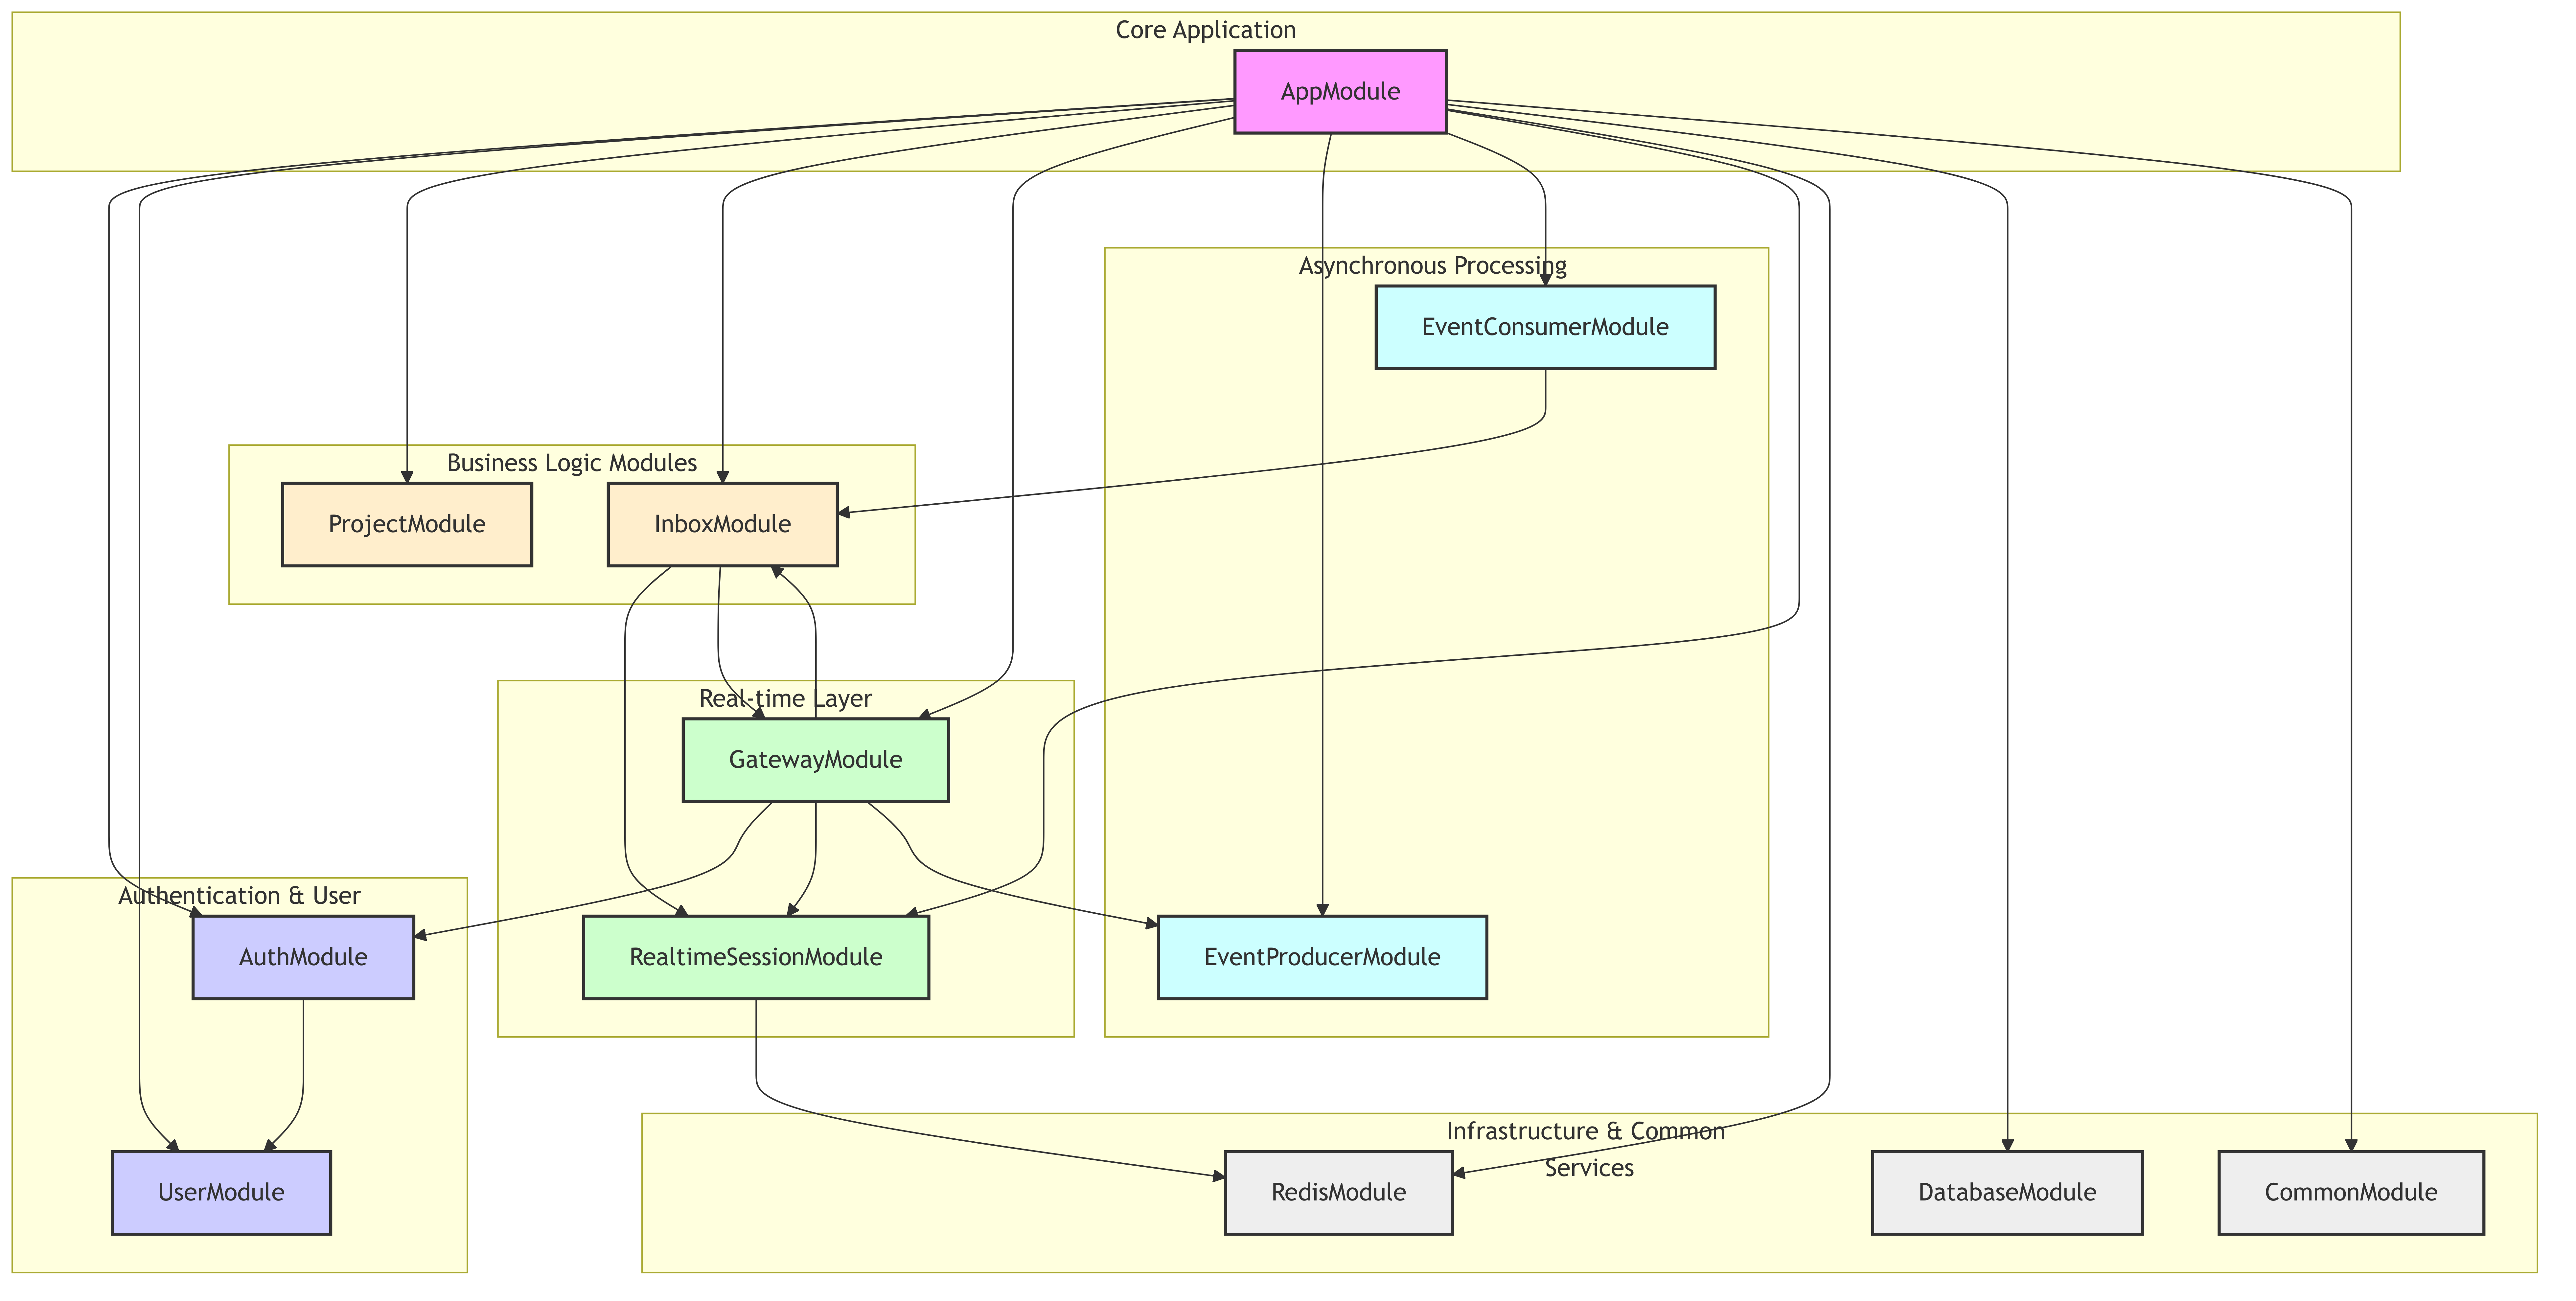
\includegraphics[width=\textwidth]{images/module-relation.png}
    \caption{Sơ đồ Phụ thuộc giữa các Module}
    \label{fig:module-dependencies}
\end{figure}
\subsection{Mô tả các Module Chính}
\label{subsec:mo-ta-module}

Dưới đây là bản tóm tắt về vai trò và trách nhiệm của từng module chính trong hệ thống, giúp làm rõ hơn chức năng của các khối trong Sơ đồ \ref{fig:module-dependencies}.

\begin{itemize}
    \item \textbf{AppModule:} Là module gốc của ứng dụng NestJS. Nó không chứa logic nghiệp vụ mà đóng vai trò là điểm tích hợp, chịu trách nhiệm "lắp ráp" và cấu hình tất cả các module khác để tạo thành một hệ thống hoàn chỉnh.

    \item \textbf{UserModule:} Quản lý tất cả các nghiệp vụ liên quan đến người dùng của hệ thống (ở đây là các nhân viên hỗ trợ - agent). Nó bao gồm các thao tác CRUD (Tạo, Đọc, Cập nhật, Xóa) thông tin người dùng và định nghĩa entity \texttt{User}.
    
    \item \textbf{AuthModule:} Chịu trách nhiệm cho toàn bộ quá trình xác thực và phân quyền. Nó xử lý logic đăng nhập, tạo và xác minh JSON Web Tokens (JWT), triển khai các cơ chế bảo vệ (Guards) cho các API endpoint. Module này phụ thuộc chặt chẽ vào \texttt{UserModule} để truy vấn thông tin người dùng trong quá trình xác thực.

    \item \textbf{ProjectModule:} Quản lý các "Dự án" của người dùng. Mỗi dự án tương ứng với một website được tích hợp widget. Module này xử lý các thao tác CRUD cho dự án và quản lý các cài đặt liên quan đến widget như domain được phép, màu sắc, câu chào.
    
    \item \textbf{InboxModule:} Là module nghiệp vụ lớn nhất, chứa toàn bộ logic cốt lõi liên quan đến Hộp thư. Nó quản lý các thực thể và nghiệp vụ của các cuộc hội thoại (\texttt{Conversation}), tin nhắn (\texttt{Message}), và khách truy cập (\texttt{Visitor}).
    
    \item \textbf{GatewayModule:} Chịu trách nhiệm cho toàn bộ giao tiếp real-time của hệ thống thông qua WebSocket (Socket.IO). Nó quản lý các kết nối từ widget và agent dashboard, xử lý các sự kiện đến và phát đi các sự kiện cập nhật cho các client liên quan.

    \item \textbf{EventProducerModule:} Một module nhỏ nhưng quan trọng trong kiến trúc bất đồng bộ. Trách nhiệm duy nhất của nó là cung cấp một service (\texttt{SqsService}) để nhận các sự kiện (ví dụ: tin nhắn mới từ visitor) và đẩy chúng vào hàng đợi SQS một cách đáng tin cậy.
    
    \item \textbf{EventConsumerModule:} Là một ứng dụng NestJS độc lập (worker), không có máy chủ HTTP. Nó lắng nghe hàng đợi SQS, nhận các sự kiện do \texttt{EventProducerModule} gửi đến và điều phối chúng đến các service nghiệp vụ tương ứng trong \texttt{InboxModule} để xử lý.

    \item \textbf{RealtimeSessionModule:} Quản lý trạng thái kết nối real-time của các visitor. Nó sử dụng Redis để lưu trữ và tra cứu mối liên kết giữa định danh của visitor (\texttt{visitorUid}) và ID kết nối socket (\texttt{socket.id}) của họ, cho phép gửi tin nhắn đến đúng người nhận.

    \item \textbf{RedisModule \& DatabaseModule:} Là các module hạ tầng. Chúng cung cấp các kết nối đã được cấu hình sẵn đến Redis và cơ sở dữ liệu PostgreSQL (thông qua TypeORM) cho toàn bộ ứng dụng.
\end{itemize}